\section{Topic Tree}
\subsection{Overview}
Most learning management systems do not have a simple and easy method to import course material and resources from other courses. Some LMS platforms such as OpenLearning have no method of importing any data at all, and other platforms such as Canvas allows you to import crowd sourced material into your own course, however still does not allow you to import topics of resources. \\

This new LMS will have a new topic tree feature, which will allow teachers and academics to add course material under a specific topic instead.\\
Each topic will have prequisites of other topics, for example the topic Graphs will be a prequisite for the topic Depth first Search.\\

\textbf{Topics} \\
A topic is a collection of educational material that is related to a particular subject. For example, in UNSW's Introduction to Programming course (COMP1511), one of the topics in the course is ``Pointers", which contains all course material related to pointers.\\

At Charles Sturt University, each topic is defined as a small subject that is three hours in length \cite{csutopictree}. CSU's curriculum covers around 1000 topics with each topic being three hours in length for a degree. In this thesis, we will also define a topic being three hours of content, but instructors can choose what amount of content constitutes as a topic.\\


\begin{figure}[h!]
    \centering
    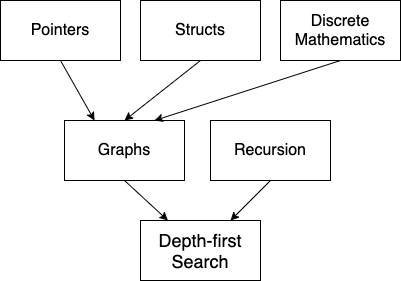
\includegraphics[scale=0.4]{topic-tree-example}
    \caption{Example of a topic tree with Depth first search}
\end{figure}

In the above example, pointers, structs and discrete mathematics must be learned in order to learn graphs. Likewise, graphs and recursion is required to learn depth first search.\\


Specific courses in this new LMS would be created by choosing the topics this new course has, and all course materials under each topic would be imported into the respective topic. This allows for faster creation of courses, and course materials can be reused more easily.\\

\subsection{UI/UX}
The UI for the topic tree involves two different views of the topic tree - a graph view and a traditional view. The graph view will be the focus of the LMS, as it will allow instructors to visualise the prerequisities between topics easily. However if time permits, a traditional interface will be implemented as well in Thesis C, with an option to switch between the two views. This traditional interface will be easier to use for some users, as it is similar to typical interfaces and a graph interface may be too confusing to use.\\

\newpage
\textbf{Graph Interface}

\begin{figure}[h!]
    \centering
    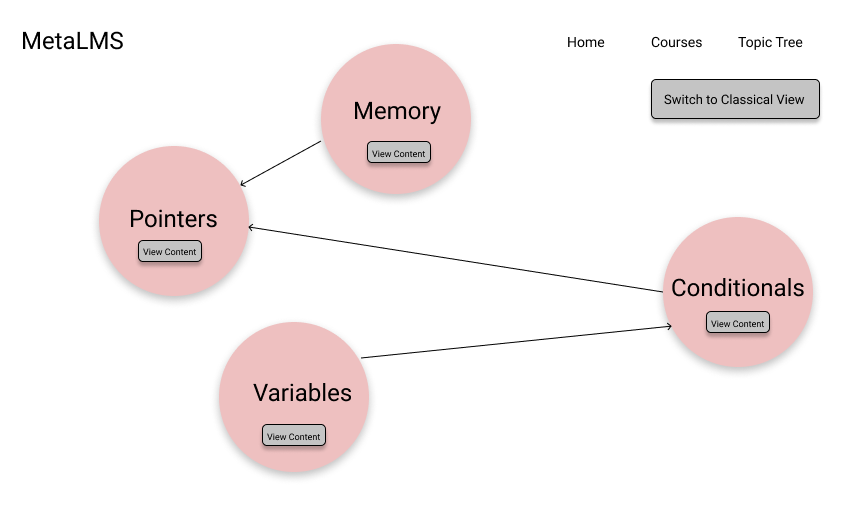
\includegraphics[scale=0.4]{topic-tree-graph-view}
    \caption{Topic Groups Graph UI}
\end{figure}

This is a mockup of a possible graph UI. Arrows indicate prerequisites, as in this example Memory is required to be learnt in order to learn about Pointers. This will be the default view of the topic tree, and a modal will open to display content for a specific topic when the ``View Content" button is clicked. Topics will be grouped together - in this example, ``Introduction to Programming" would be the name of this group of topics, and would be represented as a ``region" of the topic tree.

\textbf{Traditional Interface}\\
The following mockups show what a traditional interface could look like, and will be changed and improved upon in the future.\\
\begin{figure}[h!]
    \centering
    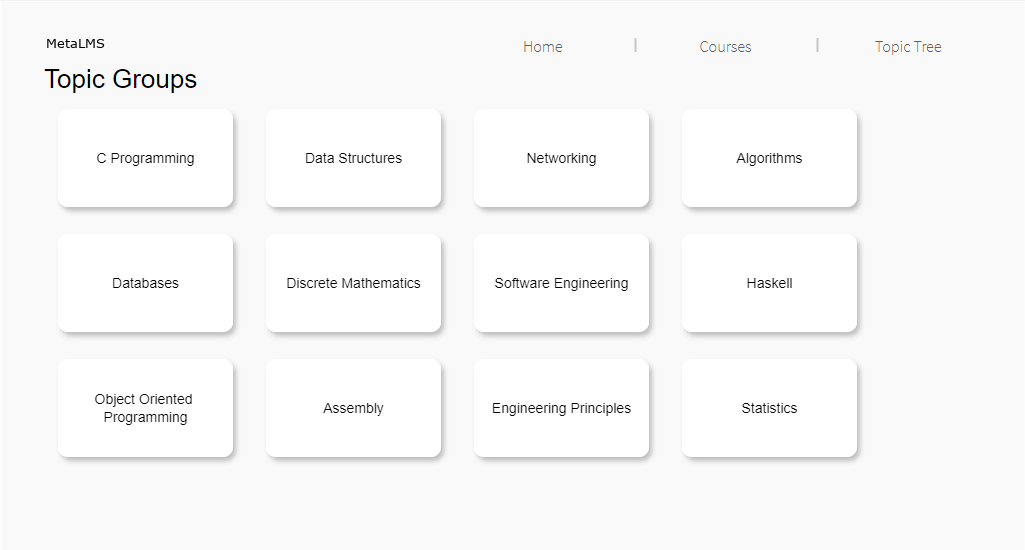
\includegraphics[scale=0.4]{topic-tree-groups-list}
    \caption{Topic Groups UI}
\end{figure}

\newpage

Each group of topics is listed in card format. The topics in each group can be viewed by clicking on the topic.\\

\begin{figure}[h!]
    \centering
    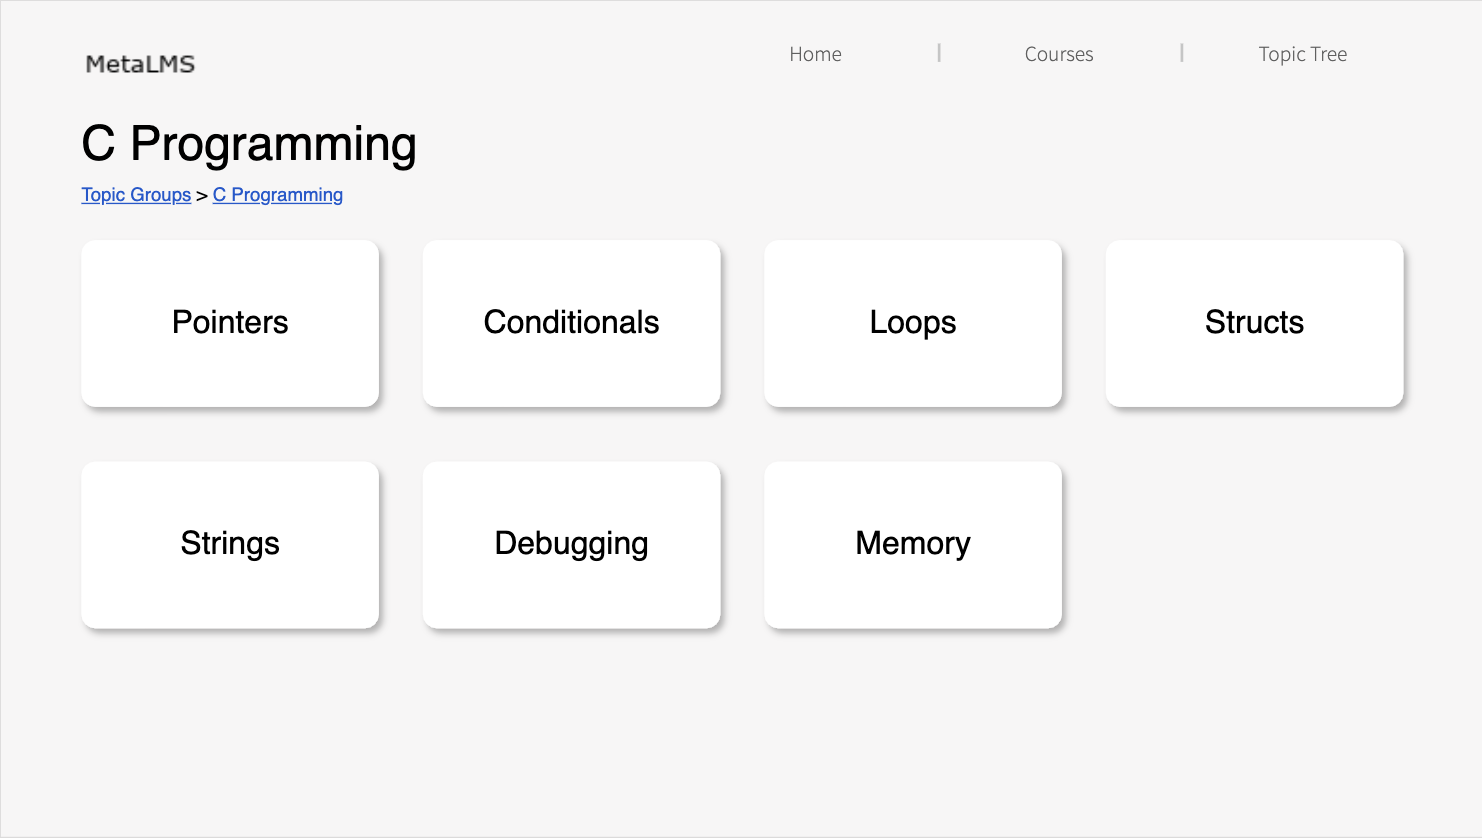
\includegraphics[scale=0.4]{topic-tree-group}
    \caption{Topic Group - C Programming Example}
\end{figure}

Inside a topic group, the full list of topics inside this group is listed. Prerequisites are NOT shown here. \\

\begin{figure}[h!]
    \centering
    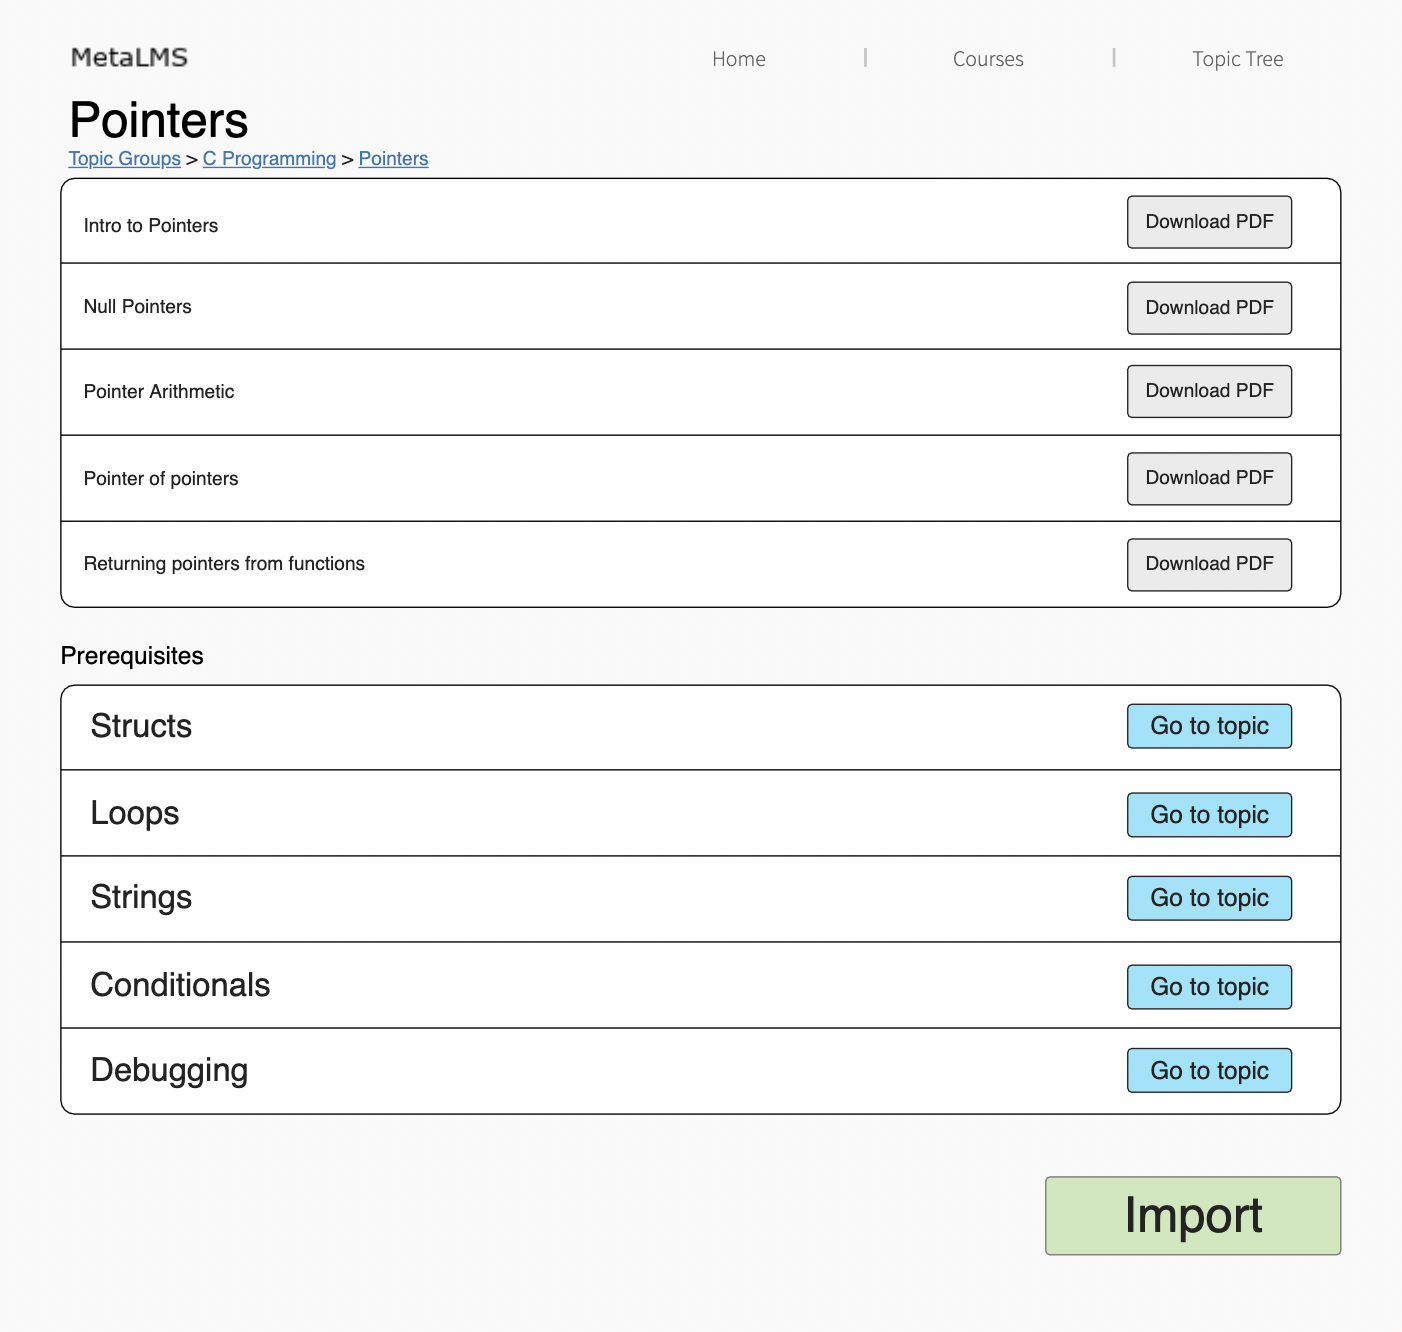
\includegraphics[scale=0.4]{topic-tree-pointers}
    \caption{Topic - Pointers Example}
\end{figure}

All resources for this topic are listed, and prerequisites are also listed on this page. This view is modelled after the UNSW Handbook \url{https://www.handbook.unsw.edu.au/}, where course prerequisites are listed as links. This topic can then be imported into a course with the import button at the bottom.\\

\subsection{Requirements}
The requirements below are draft requirements, and will become more specific throughout the next stages of the thesis.\\
Each requirement will have a priority: High, Medium or Low. High priority requirements will be completed first, and then medium and low priority requirements respectively. \\

\subsection{Functional Requirements}

\textbf{Viewing Topics}

    \begin{enumerate}
    \item Users can view groups of topics \textcolor{Orange}{Medium}
    \item Users can view topics within each group \textcolor{Red}{High}
    \item Users can search for a topic \textcolor{Red}{High}
    \item Users can search for specific resources \textcolor{Red}{High}
    \item Users can view topic prerequisites \textcolor{Orange}{Medium}
    \item Users can view a graph of topics and their prerequisites \textcolor{Red}{High}
    \item Users can view the topic tree with a traditional interface \textcolor{Blue}{Low}
    \end{enumerate}

\textbf{Adding Topics and resources}
    \begin{enumerate}
    \item Users can add a new topic \textcolor{Red}{High}
    \item Users can upload course material \textcolor{Red}{High}
    \item Users can add a new topic group \textcolor{Orange}{Medium}
    \end{enumerate}

\textbf{Deleting Topics}
    \begin{enumerate}
    \item Users can delete a topic that they've created \textcolor{Red}{High}
    \item Users can delete a topic group that they've created \textcolor{Orange}{Medium}
    \item Users can remove course material from a topic \textcolor{Red}{High}
    \end{enumerate}

\textbf{Topic Prequisites}
    \begin{enumerate}
    \item Users can add a topic prerequisite \textcolor{Orange}{Medium}
    \item Users can delete a topic prerequisite \textcolor{Orange}{Medium}
    \end{enumerate}

\textbf{Integration}
    \begin{enumerate}
    \item Users can import course material by selecting topics for a course \textcolor{Red}{High}
    \item Users can remove topics from a course \textcolor{Red}{High}
    \end{enumerate}

\textbf{Exporting}
    \begin{enumerate}
    \item Users can export data from topics and course material \textcolor{Blue}{Low}
    \end{enumerate}

\subsection{Timeline}
This timeline details what is planned over the course of the year to achieve a working topic tree feature in the meta learning management system.
Milestones are featured throughout this timeline.

\newpage

\begin{figure}[h!]
    \centering
    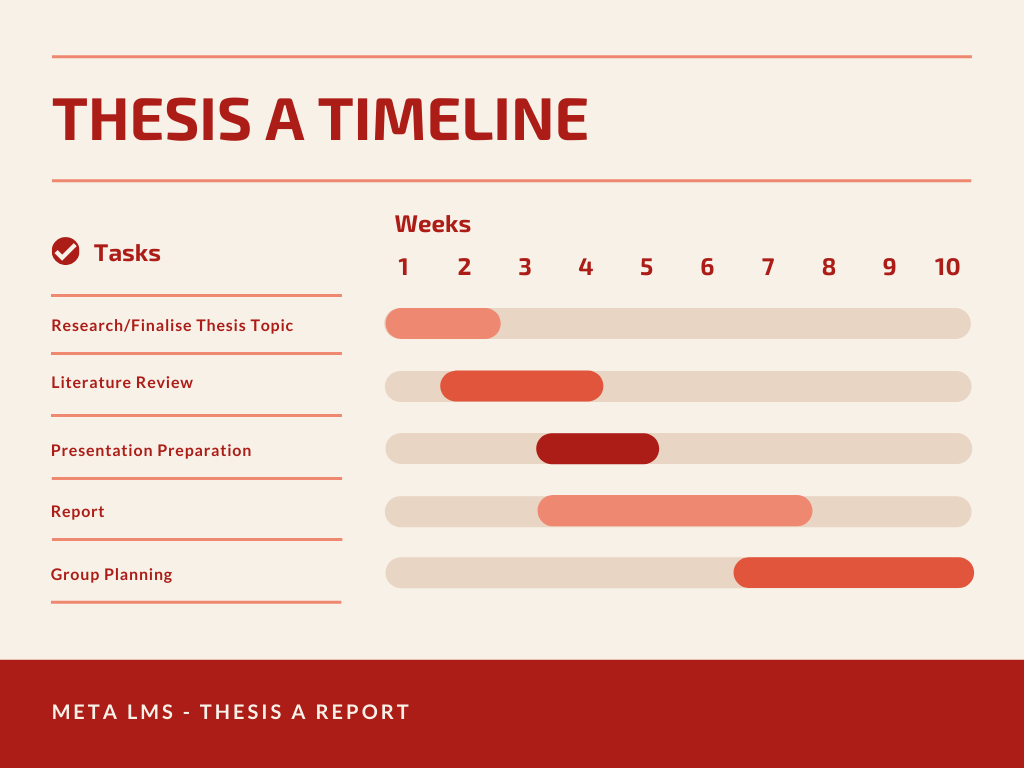
\includegraphics[scale=0.4]{topic-tree-thesis-a}
    \caption{Thesis A Timeline}
\end{figure}

This term, the focus is literature review and planning features for implementation in Thesis B and C.


\begin{figure}[h!]
    \centering
    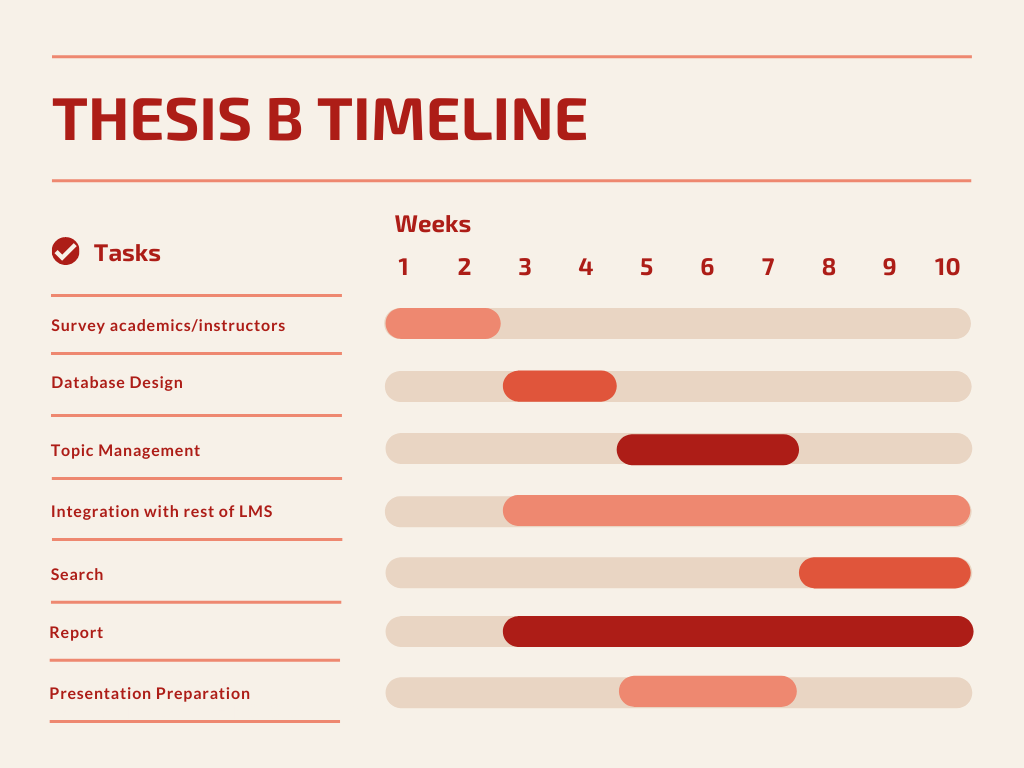
\includegraphics[scale=0.4]{topic-tree-thesis-b}
    \caption{Thesis B Timeline}
\end{figure}

In Thesis B, the focus is to start implementing the topic tree feature, with core features implemented and mostly usable including the graph interface, and a working database design. \\

Database Design will involve designing a schema for the database to store topics and their dependencies. This will most likely involve a graph relationship between topics.\\
Topic Management involves designing the graph interface for adding, removing and managing topics and helping develop a backend for this.\\
Integration with the rest of the system involves using the topic tree to import content into a course, and export content into the topic tree, etc.\\
Search involves searching for content, and is not as important as developing the topic management feature.\\
A graph interface would make it much easier to visualise dependencies between topics, but is not a high priority so the plan is to implement this during Term 2 2021.\\

\begin{figure}[h!]
    \centering
    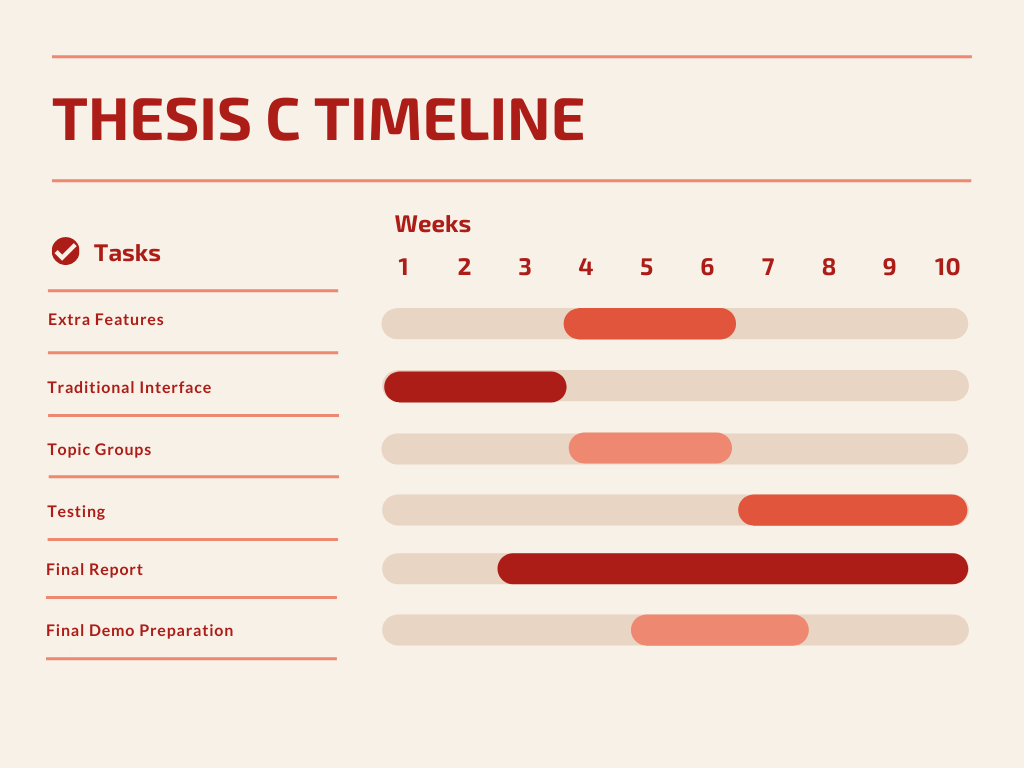
\includegraphics[scale=0.4]{topic-tree-thesis-c}
    \caption{Thesis C Timeline}
\end{figure}

In Thesis C, the main focus is to finalise features, fix any bugs that arise, test the feature and its integration with the rest of the system, implement a traditional interface and allow topics to be grouped with each other.\\

A traditional interface would be easier to use than a graph interface for some users, as it would be more similar to most interfaces used in other software, and would be implemented during Term 3 2021.\\

\newpage
\subsection{Milestones}
Major milestones for the topic tree feature include: \\
\begin{enumerate}
\item Week 6 Term 2 2021 - Implement a database schema for storing topics and their prerequisites, and set up a graph interface for topic management to easily view prerequisites between topics and topic groups.
\item Week 11 Term 2 2021 - Adding and deleting topic prerequisites/dependencies, a search function and proper integration with the rest of the learning management system.
\item Week 6 Term 3 2021 - Traditional interface to improve the user experience of the LMS.
\item Week 11 Term 4 2021 - Final Testing and Analysis of the learning management system.
\end{enumerate}

\subsection{Evaluation}
In order to evaluate how well the feature has met its requirements and achieved its purpose, a criteria will be proposed. \\

This feature will be evaluated in several areas:\\
\textbf{Functional Requirements} \\
The feature must meet all of its functional requirements to ensure that the feature is complete and meets its purpose. Higher priority requirements must be completed before lower priority requirements. Testing tools and data will be used in order to assess its functionality, using tools such as React Testing Library \cite{reactTestingLibrary} and Insomnia Unit Testing \cite{insomniaTesting}.\\

\textbf{Performance} \\
Performance must be high and the feature must be responsive to provide a high quality user experience for both academics and students. Performance will be assessed using tools such as Google Lighthouse \cite{googleLighthouse}. Google Lighthouse uses several metrics to assess performance, as explained previously. \\

\textbf{Accessibility} \\
The topic tree feature will also be assessed on how accessible the interface is. If features such as alt tags, high contrast colours and keyboard navigation are not implemented then not all academics and students will be able to use the topic tree feature. Therefore, tools such as Google Lighthouse will be used to access its accessibility as the tool also includes metrics for measuring accessibility of a website \cite{googleLighthouseAccessibility}. \\

\textbf{Usability} \\
Finally, the feature will be assessed on its usability. This includes whether the topic tree feature is attractive and easy to use. Various students and academics will be surveyed on how easy they found the system to use. The number of errors and time taken to complete a task will also be assessed.\\
